\section{Návrh uživatelského rozhraní - Lo-Fi prototyp}

V poděkování jsem zmiňoval, že při prvotním návrhu UI jsme spolupracovali jako tým v předmětu MI-NUR. Tento tým byl vytvořen přímo za účelem realizace prototypu skladového systému, na kterém jsem následně chtěl dále pracovat již v rámci této diplomové práce. Proto jsem byl zvolen vedoucím týmu, staral se o kvalitu našeho týmového výstupu a sledoval pozorně i části, které zpracovávali mí kolegové, protože jejich výstup přímo napomáhal vyšší kvalitě mé navazující práce. V rámci týmu jsme se pro zjednodušení zaměřili především na pohled role skladníka.\\
První částí návrhu GUI byl mockup, či chcete-li wireframe. Pro jeho tvorbu jsme využili nástroj Axure RP \cite{axure} - jedná se o komplexní nástroj pro tvorbu prototypů, bez nutnosti psaní programového kódu. Lze do něj doinstalovat externí knihovny, které například přidávají hotové designové či funkční prvky, a má vlastní řešení kolaborace a verzování ve stylu SVN.\\
Pro naše potřeby jsme tedy do Axure doinstalovali UX Tool Time \cite{uxtooltime}, což je knihovna pro Axure, která nabízí komponenty v \emph{Material designu}. S její pomocí jsme vytvořili návrhy na základní procesy skladníka.\\

\begin{figure}[]
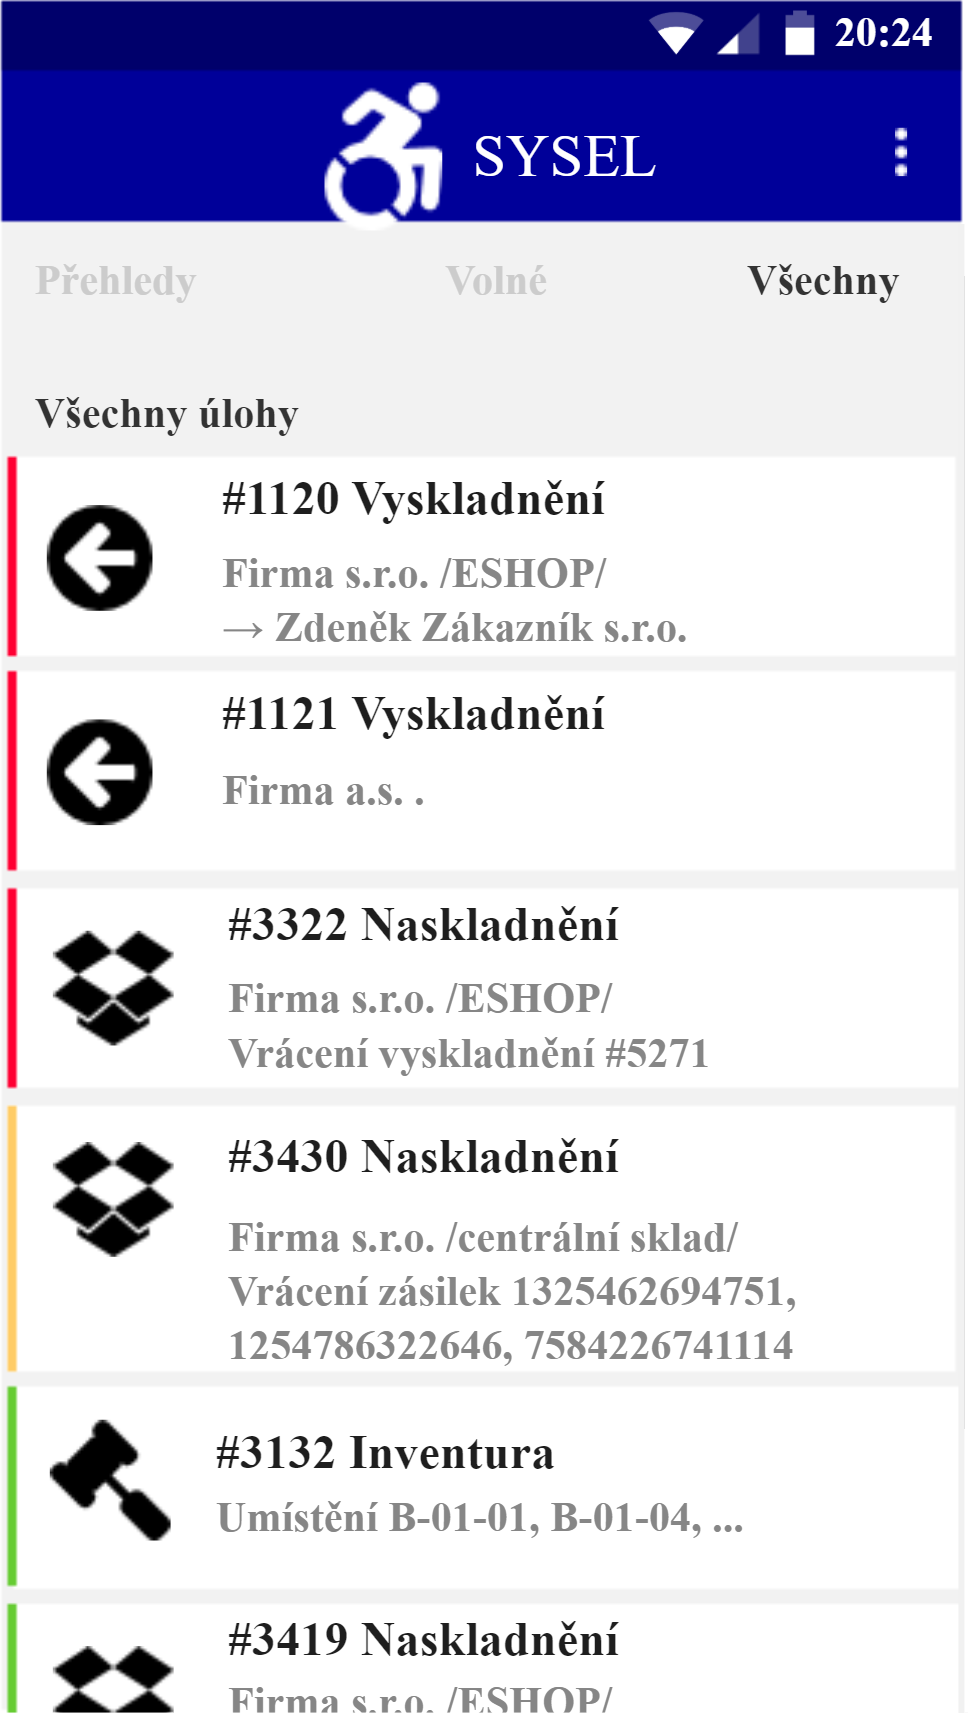
\includegraphics[height=0.6\textheight]{../png/axure/homepage.png}
\caption{Domovská obrazovka aplikace: Lo-Fi prototyp} \label{picture:axure:homepage}
\end{figure}

\paragraph{Domovská obrazovka.} Právě ve fázi návrhu Lo-Fi prototypu jsem rozhodl o novém základním rozložení obrazovek v systému - vertikální řazení veškerých položek, které již bylo znázorněno v předchozí kapitole na obrázku \ref{picture:sysel:vertical} bylo přepracováno do více pohledů, které se na velké obrazovce mohou zobrazovat vedle sebe, na mobilním zařízení pak mezi nimi bude možné přecházet posunem - zárodek tohoto řešení je vidět na obrázku \ref{picture:axure:homepage}, jedná se o texty \uv{Přehledy}, \uv{Volné} a \uv{Všechny} v horní části obrazovky. Obsah, který se bude na jednotlivých pohledech zobrazovat, by mohl být konfigurovatelný a uživatel by si tak mohl nastavit přesně ty seznamy, které ho zajímají. Kromě toho je také na vložené ukázce vidět první verze znázornění priorit - levý okraj karet úkolů nabývá zelené, žluté a červené barvy podle nastavené priority úkolu.

\begin{figure}[h]
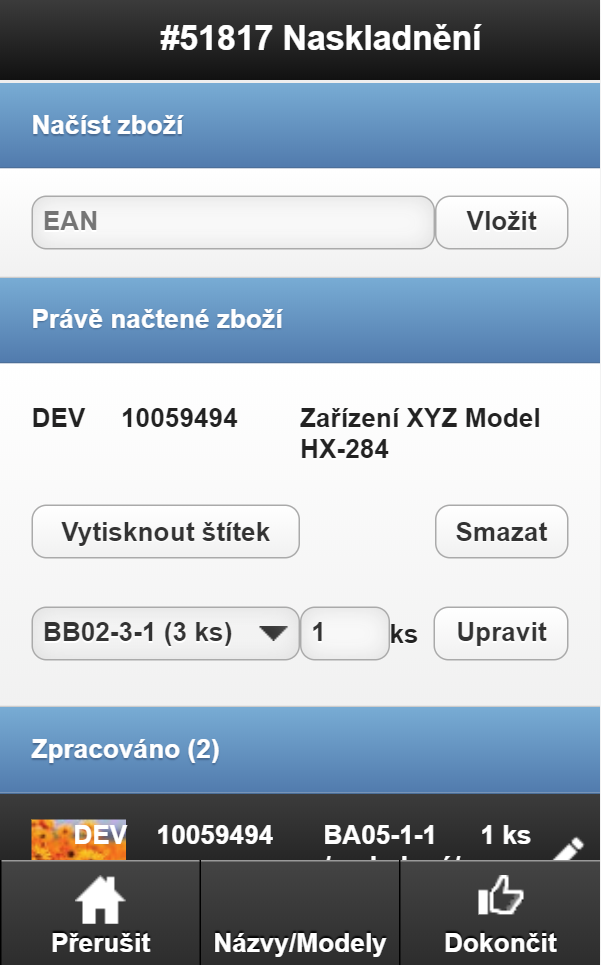
\includegraphics[height=0.6\textheight]{../png/sysel/naskladneni.png}
\caption{Rozhraní skladníka pro naskladňování položek: starý skladový systém} \label{picture:sysel:naskladneni}
\end{figure}

\paragraph{Naskladnění.} Další ukázkou z této fáze je obrazovka naskladnění - do textu je vložena jako obrázek \ref{picture:axure:naskladneni}, pro porovnání je vložena i ukázka starého skladového systému - obrázek \ref{picture:sysel:naskladneni}. V novém systému je v této fázi vidět ještě poměrně silná inspirace rozpoložení ve starém systému a návrh je tak spíše pouze oblečen do modernějšího designu. Dokončení úlohy je v pravém horním rohu, kde je sice stále na očích, ale, jak jsem zjistil později a také při zpětném pohledu na analýzu konkurenčních řešení, toto řešení není příliš vhodné kvůli své nevýraznosti, a tak bylo ještě v další iteraci přepracováno.\\

\begin{figure}[h]
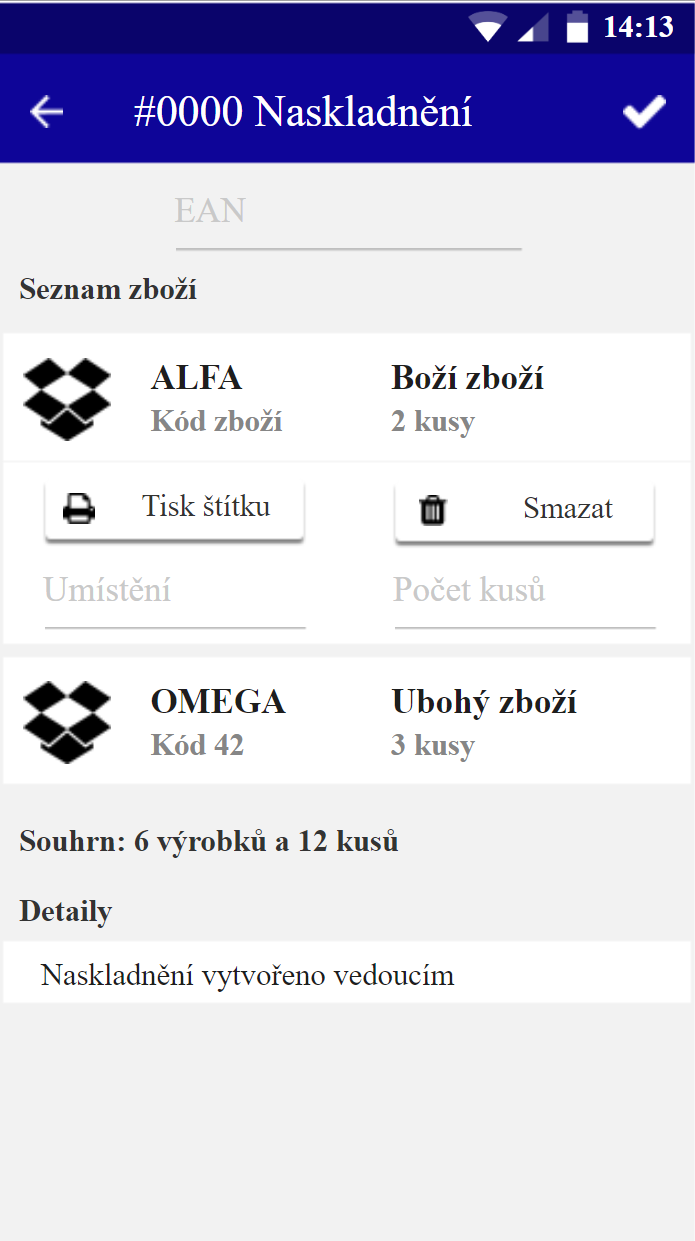
\includegraphics[height=0.6\textheight]{../png/axure/naskladneni.png}
\caption{Rozhraní skladníka pro naskladňování položek: Lo-Fi prototyp} \label{picture:axure:naskladneni}
\end{figure}

\begin{figure}[h]
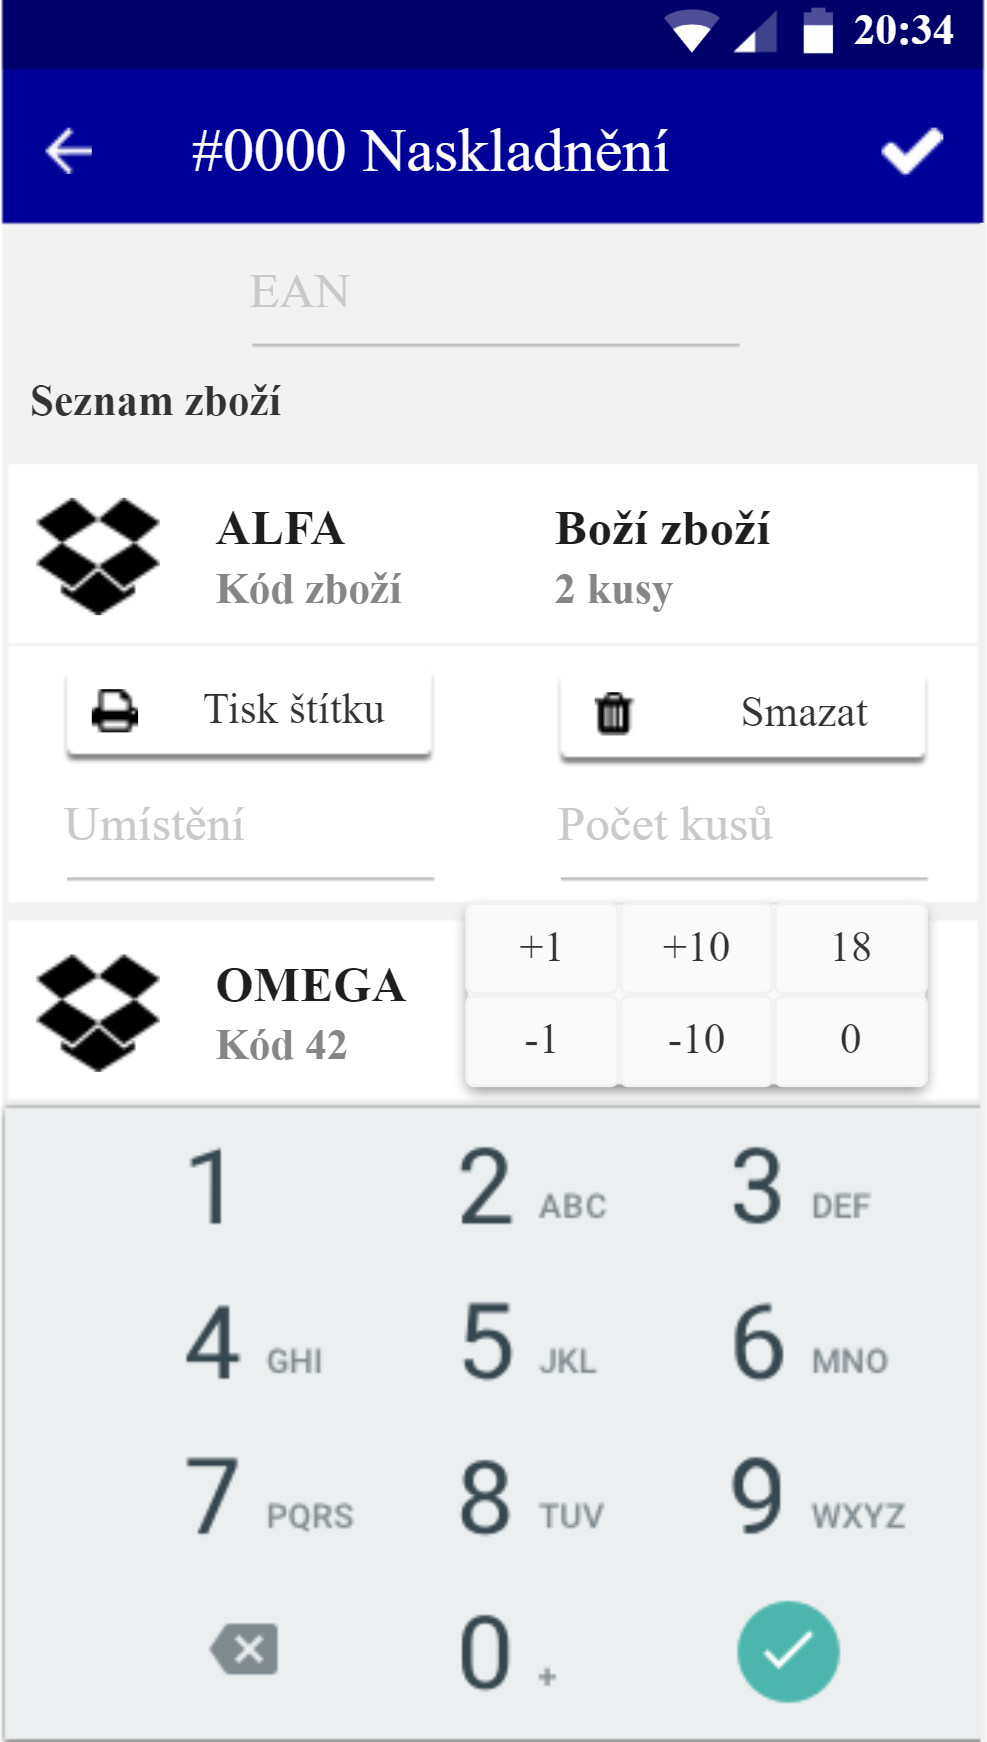
\includegraphics[height=0.6\textheight]{../png/axure/keyboard.png}
\caption{Naskladňování - rychlé zadání počtu kusů zboží: Lo-Fi prototyp} \label{picture:axure:keyboard}
\end{figure}

\paragraph{Zadávání počtu kusů.} Novinkou, která se objevila již v Lo-Fi prototypu je snadnější zadávání počtu kusů zboží, pro které jsem vložil samostatnou ukázku jako obrázek \ref{picture:axure:keyboard}, umožňující jak přímo zadání počtu kusů, tak i možnost přeskakovat po jednom nebo deseti kusech, ve směru nahoru i dolů. Tento výběr se zobrazuje při aktivním poli \uv{Počet kusů}, které bohužel na vloženém obrázku nevypadá aktivně, protože to Lo-Fi prototyp nepodporoval.\\

Kompletní zdrojové kódy Lo-Fi prototypu jsou k dispozici na přiloženém médiu.\\
Lo-Fi prototyp byl zkontrolován odbornou osobou a na základě získané zpětné vazby proběhla další iterace - návrh Hi-Fi prototypu.\\
